\section{06.11.23 : Lemat o wężu i przyjaciele (kwadraty kartezjańskie)}

Na tym wykładzie trzymamy z tyłu głowy, że jesteśmy w kategorii abelowej.

\subsection{Epimorfizm (i jądro) przenosi się przez pull-back}

\begin{lemma}[epimorfizm przenosi się przez pull back]\label{epi przez pull back}
  Jeśli mamy dany pull-back (kwadrat kartezjański, tzn. $Z$ wraz z $g'$ i $g$ jest granicą początku alfabetu)
  \begin{center}\begin{tikzcd}[column sep=large]
    Z\arrow[r, "f'"]\arrow[d, "g'" left] & B\arrow[d, "g"] \\ 
    A\arrow[r, "f" below] & C
  \end{tikzcd}\end{center}
  wtedy jeśli $f$ jest epimorfizmem, to $f'$ też takie jest.
\end{lemma}

\begin{proof}
  Zaczniemy naszą przygodę od powiększenia diagramu tak, aby było widać jak konstruowany jest pull-back.

  \begin{center}\begin{tikzcd}[column sep=large]
    Z\arrow[rr, "f'"]\arrow[dd, "g'" left]\arrow[dr, "m"] & & B\arrow[dd, "g"]\arrow[dl, "i_B" below, yshift=-1mm]\\ 
                                                          & A\oplus B\arrow[ur, "P_B" above, yshift=1mm] \arrow[dl, "P_A" above, yshift=1mm] \arrow[dr, "fP_A-gP_B" above right] \\ 
    A \arrow[ur, "i_A" below, yshift=-1mm] \arrow[rr, "f" below] &  & C
  \end{tikzcd}\end{center}
  Wiemy, że $m$ jest jądrem odwzorowania $(fP_A-gP_B)$, czyli musi być monomorfizmem. Przejdziemy przez kilka etapów, żeby wyciągnąć bycie epimorfizmem przez $f$ do bycia epimorfizmem przez $f'$.
  \begin{enumerate}
    \item $f$ jest epimorfizmem $\implies fP_A-gP_B$

      Weźmy sobie dowolny $D$ i wyobraźmy sobie, że mamy strzałkę $\alpha:C\to D$ taka, że $\alpha(fP_A-gP_B)=0$. Musimy więc pokazać, że wtedy $\alpha$ musi być $0$.
      \begin{align*}
        0 &= \alpha(fP_A-gP_B)i_A=\alpha f\overbrace{P_Aid_A}^{id_A}-\alpha g\overbrace{P_Bid_A}^0=\\ 
          &=\alpha f\;id_A=\alpha f
      \end{align*}
      Skoro więc $\alpha f=0$, a $f$ jest epimorfizmem, to na pewno wiemy, że $\alpha=0$.
    \item $f'$ jest epimorfizmem

      Wyobraźmy sobie, że teraz z kolei istnieje $E$ oraz strzałka $h:B\to E$ taka, że $hf'=0$. Tak jak wcześniej, musimy pokazać, że $h=0$.

      Zauważmy, że $f'=P_Bm$, czyli możemy napisać
      $$0=hf'=hP_Bm$$
      czyli $hP_B$ faktoryzuje się przez $\coker m$, ale czym tak właściwie jest $\coker m$? Otóż $\coker m=C$! W takim razie możemy znaleźć $h':C\to E$ takie, że
      $$h'(fP_A-gP_B)=hP_B,$$
      czyli znowu szukając zera dostaniemy
      \begin{align*}
        0&=h\overbrace{P_Bi_A}^0=h'(fP_A-gP_B)i_A=\\ 
         &=h'fP_Ai_A-h'gP_Bi_A=h'f
      \end{align*}
      Wiemy, że $f$ jest epimorfizmem, czyli $h'=0$. W takim razie
      $$0=h'(fP_A-gP_B)=hP_B$$
      ale z drugiej strony $h=hP_Bi_B$, czyli mamy
      $$h=hP_Bi_B=0i_B=0$$
      i dostajemy to co chcieliśmy.
  \end{enumerate}
\end{proof}

\begin{lemma}[jądro przenosi się przez pull-back]
  Rozważamy diagram
  \begin{center}\begin{tikzcd}
    K\arrow[r, "k"]\arrow[dr, "g'k" below left, dashed]& Z\arrow[r, "f'"]\arrow[d, "g'"] & B\arrow[d, "g"]\\ 
                    & A\arrow[r, "f"] & C
  \end{tikzcd}\end{center}
  gdzie $K\xrightarrow{k}Z$ jest jądrem $f'$. Wówczas $K\xrightarrow{g'k}A$ jest jądrem $f$.
\end{lemma}

\begin{proof}
  Musimy pokazać, że $fg'k=0$ oraz że takie $g'k$ spełnia warunek uniwersalności.

  \begin{itemize}
    \item $fg'k=0$

      Wystarczy zobaczyć rysunek:
      \begin{center}\begin{tikzcd}
        K\arrow[r, "k" below]\arrow[rr, "0" above, bend left=20]\arrow[drr, rounded corners, thick, to path ={ ([yshift=1mm]\tikztostart.south) -| ([xshift=10mm, yshift=-2mm]\tikztostart.south) |- ([yshift=-10mm]\tikztotarget)}, orange]\arrow[drr, rounded corners, thick, to path ={ -| ([yshift=4mm]\tikztostart.north) -| ([xshift=15mm]\tikztotarget)}, green]
        & Z\arrow[r, "f'" below]\arrow[d, "g'"{coordinate, name=Z}] & B\arrow[d, "g"]\\ 
        & A\arrow[r, "f"] & C
      \end{tikzcd}\end{center}
      Zielona strzałka na górze jest złożeniem funkcji $0$ z $g$, czyli sama jest $0$, a ponieważ pomarańczowa strzałka niżej jest jej równa (diagram komutuje), to ona również jest zerem.

    \item $g'k$ spełnia uniwersalną własność jądra

      Niech $U$ będzie takie, że $fu=0$. Wtedy możemy narysować diagram z którego wynika, że $U$ jest stożkiem nad diagramem \begin{tikzcd}A\arrow[r, "f"] & C & \arrow[l, "g"] B\end{tikzcd}
      \begin{center}\begin{tikzcd}[column sep=large, row sep=large]
        U\arrow[r, "0" above]\arrow[d, "u" left]\arrow[dr, "fu=0" above right] & B\arrow[d, "g" right]\\ 
        A\arrow[r, "f" below] & C
      \end{tikzcd}\end{center}

      Z uniwersalności $Z$ jako granicy diagramu \begin{tikzcd}A\arrow[r] & C & B\arrow[l]\end{tikzcd} możemy dostać jedyną strzałkę $\exists! u'U\to Z$, która daje diagram:

      \begin{center}\begin{tikzcd}[column sep=large, row sep=large]
    K\arrow[r, "k"]& Z\arrow[r, "f'"]\arrow[d, "g'"] & B\arrow[d, "g"]\\ 
    U\arrow[r, "u" below] \arrow[ur, "\exists! u'" left]\arrow[u, "\exists! u''?", left, dashed] & A\arrow[r, "f" below] & C
  \end{tikzcd}\end{center}

  Wystarczy zauważyć, że $K$ jest jądrem strzałki $gf'$ oraz że $gf'u'=0$, czyli $u'$ faktoryzuje się przez $K$:
  $$gfu'=fg'u'=fu=0.$$
  Stąd mamy istnienie jedynej strzałki $u''$ jak na diagramie.

  %{\large\color{red}DO DOKOŃCZENIA}
  \end{itemize}
\end{proof}

\subsection{Czym są elementy obiektu?}

\begin{definition}[element obiektu]
  Jeśli $\mathbf{A}$ jest kategorią abelową i $Y\in\ob \mathbf{A}$, to elementem $Y$ nazywamy \buff{klasę równoważności morfizmów} $X\xrightarrow{h}Y$ względem relacji
  \begin{center}\begin{tikzcd}[row sep=small, /tikz/column 2/.style={column sep=0.2mm}, /tikz/column 1/.style={column sep=0.2mm}]
    (X\xrightarrow{h}Y) & \sim \arrow[d, sloped, phantom, "\iff"] & (X'\xrightarrow[h'] Y) \\ 
    (\exists u, u':Z\twoheadrightarrow X)& Z\arrow[r, "u"] & X\\ 
                          & Z\arrow[r, "u'"] & X'\\ 
                      & hu=h'u'
  \end{tikzcd}\end{center}
  to znaczy, że istnieją $u, u'$ epimorfizmy takie, że komutuje diagram
  \begin{center}\begin{tikzcd}
    & Z\arrow[dr, "u"]\arrow[dl, "u'" above left] \\ 
    X \arrow[dr, "h" below left] & & X'\arrow[dl,"h'"]\\ 
                      & Y 
  \end{tikzcd}\end{center}
\end{definition}

Powyższa relacja jest relacją równoważności, bo biorąc $Z''$ jako pullback 
\begin{center}\begin{tikzcd}[column sep=small]& Z'\arrow[d]\\ Z\arrow[r] & X'\end{tikzcd}\end{center}
oraz korzystając z lematu \ref{epi przez pull back}, dostajemy przemienny diagram

\begin{center}\begin{tikzcd}
  & & {\color{orange}Z''}\arrow[dr, orange]\arrow[dl, orange]\\ 
  & Z\arrow[dr]\arrow[dl] & & Z'\arrow[dr]\arrow[dl]\\ 
  X\arrow[drr] & & X'\arrow[d] & & X''\arrow[dll]\\ 
              & & Y
\end{tikzcd}\end{center}

O elementach możemy nadal myśleć jako o elementach "zbioru" $Y$ i podmieniać to myślenie na klasy abstrakcji relacji wyżej, jeśli jest to dla nas bardziej wygodne.

{\large\bfseries\color{green}Własności elementów $\mathbf{Y}$}

\begin{enumerate}
  \item Odwzorowanie $Y\xrightarrow{f}Y'$ jest monomorfizmem $\iff$ dla wszystkich elementów $y\in Y$ $f(y)=0\implies y=0$ $\iff$ dla dowolnych $y_1,y_2\in Y$ jeśli $f(y_1)=f(y_2)\implies y_1=y_2$.
  \item $Y\xrightarrow{f}Y'$ jest epimorfizmem $\iff$ dla każdego $y'\in Y'$ istnieje $y\in Y$ taki, że $f(y)=y'$.
  \item $Y\xrightarrow{f}Y'$ jest odwzorowaniem zerowym $\iff$ $(\forall y\in Y)\;f(y)=0$
  \item Ciąg \begin{tikzcd}Y\arrow[r, "f"] & Y'\arrow[r, "g"] & Y''\end{tikzcd} jest dokładny $\iff$ $gf=0$ oraz dla każdego $y'\in Y'$ takiego, że $g(y')=0$ istnieje $y\in Y$ taki, że $y'=f(y)$.
\end{enumerate}

\begin{proof}
  Najpierw zastanówmy się, co to znaczy, że $y=0$?
  \begin{center}\begin{tikzcd}
    & Z\arrow[dr, "0"]\arrow[dl, "u" above left] \\ 
    X\arrow[dr, "y" below left] & & 0\arrow[dl, "0"]\\ 
                     & Y
  \end{tikzcd}\end{center}
  Skoro $y=0$, to powyższy diagram komutuje. Wiemy, że $u$ jest epimorfizmem oraz $yu=0$, więc $y=0$. Czyli $y=0$ jako normalny element $\iff$ $y=0$ jako morfizm.

  Pokażemy punkt $1$, tzn. $f$ jest monomorfizmem $\iff$ dla wszystkich elementów $y\in Y$ $f(y)=0\implies y=0$.

  $\implies$ jeśli \begin{tikzcd}Y\arrow[r, "f"] & Y'\end{tikzcd} jest monomorfizmem oraz $f(y)=0$, to możemy narysować
  \begin{center}\begin{tikzcd}
    X\arrow[d, "y" left]\arrow[dr, "0"]\\ 
    Y\arrow[r, "f" below] & Y'
  \end{tikzcd}\end{center}
  Z niego wiemy, że $fy=0$, a skoro $f$ jest monomorfizmem, to $y=0$ jako morfizm. Wcześniej pokazaliśmy, że $y=0$ jako morfizm $\iff$ $y=0$ jako element. Czyli dostajemy to czego oczekiwaliśmy.

  $\impliedby$

  Zakładamy, że $fy=0$ i pytamy, czy wynika z tego, że $f$ jest monomorfizmem? Wiemy, że $fy=0\implies y=0$ jako element, ale $y=0$ jako element $\iff$ $y=0$ jako morfizm. Czyli $fy=0\implies y=0$ oznacza, że $f$ spełnia warunek na monomorfizm. 
\end{proof}

\subsection{Lemat o wężu 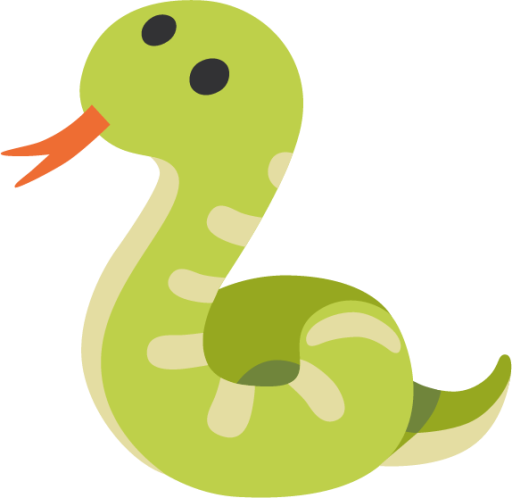
\includegraphics[width=4mm]{wunsz.png}}

\begin{definition}[ciąg dokładny]
  W kategorii abelowej kompleks łańcuchowy
  \begin{center}\begin{tikzcd}
    A^\cdot & ... \arrow[r] & A^{i-1} \arrow[r, "d^{i-1}"] & A^i\arrow[r, "d^i"] & A^{i+1} \arrow[r] & ...
  \end{tikzcd}\end{center}
  jest dokładny w $A^i$, jeśli $d^id^{i-1}=0$ oraz $i$-ta grupa kohomologii $H^i(A^\cdot)=0$.

\end{definition}

\begin{lemma}
  Ciąg jest dokładny w $A^i$ $\iff$ $\img d^{i-1}=\ker d^i$.
\end{lemma}

\begin{proof}
  $\impliedby$ 
  Wiemy, że $\img d^{i-1}=\ker d^i$, czyli narysujmy diagram
  \begin{center}\begin{tikzcd}[column sep=large, row sep=large]
    & & C\arrow[d, "b", dashed]\\
    A^{i-1}\arrow[r, "d^{i-1}"]\arrow[dr, "a\;epi" below left, dashed] & A^i \arrow[r, "d^i"]\arrow[ur, "c"] & A^{i+1}\\ 
                                & K\arrow[u, "k\;mono" right]
  \end{tikzcd}\end{center}
  {\large\color{red}WRÓCIĆ}
\end{proof}

\begin{example}
  \item Ciąg \begin{tikzcd}0\arrow[r] & A\arrow[r, "f"] & B\end{tikzcd} jest dokładny $\iff$ $f$ jest monomorfizmem 
  \item Ciąg \begin{tikzcd}A\arrow[r, "f"] & B\arrow[r] & 0\end{tikzcd} jest dokładny $\iff$ $f$ jest epimorfizmem 
  \item Jeśli mamy ciąg \begin{tikzcd}0\arrow[r] & A\arrow[r, "f"] & B\arrow[r] & 0\end{tikzcd} to jest on dokładny $\iff$ $f$ jest izomorfizmem
  \item Klasyczny ciąg dokładny to:
    \begin{center}\begin{tikzcd}
      0\arrow[r] & A\arrow[r, "f"] & B\arrow[r, "g"] & C\arrow[r] & 0 
    \end{tikzcd}\end{center}
    gdzie $f$ jest monomorfizmem, a $g$ jest epimorfizmem.
\end{example}

\begin{lemma}[o wężu]
  Załóżmy, że dany jest diagram
  \begin{center}\begin{tikzcd}
    & A\arrow[r]\arrow[d, "\alpha"] & B\arrow[r]\arrow[d, "\beta"] & C\arrow[r]\arrow[d, "\gamma"] & 0\\ 
    0 \arrow[r] & A'\arrow[r] & B' \arrow[r] & C'
  \end{tikzcd}\end{center}
  gdzie wiersze są dokładne, a wszystkie kwadraty komutują.

  Wtedy istnieje odwzorowanie $\ker\gamma\to\coker\alpha$ takie, że ciąg 
  \begin{center}\begin{tikzcd}
    \ker\alpha\arrow[r] & \ker\beta\arrow[r]\arrow[d, phantom, ""{coordinate, name=Z}] & \ker\gamma
    \arrow[dll, rounded corners, to path={ -- ([xshift=2ex]\tikztostart.east) |- (Z) [near end]\tikztonodes -| ([xshift=-2ex]\tikztotarget.west) -- (\tikztotarget) }] \\ 
    \coker\alpha\arrow[r] & \coker\beta \arrow[r] & \coker\gamma 
  \end{tikzcd}\end{center}
  jest dokładny.
\end{lemma}

\begin{proof}
  Dowód to polowanie po diagramie, którego nie będę pisać. Narysuję za to bardziej czytelny diagram:
  \begin{center}\begin{tikzcd}
   &  \color{orange} \ker\alpha \arrow[r]\arrow[d] & \color{orange} \ker\beta \arrow[r]\arrow[d] & \color{orange} \ker\gamma \arrow[d]
    \arrow[dddll, rounded corners, to path={ -- ([xshift=2ex]\tikztostart.east) |- (Z) [near end]\tikztonodes -| ([xshift=-2ex]\tikztotarget.west) -- (\tikztotarget) }, orange, thick] \\  
   & A\arrow[d, "\alpha"]\arrow[r] & B\arrow[r]\arrow[d, "\beta"]\arrow[d, phantom, ""{coordinate, name=Z}] & C \arrow[r]\arrow[d, "\gamma"] & 0\\ 
    0\arrow[r] & A'\arrow[r]\arrow[d] & B'\arrow[r]\arrow[d] & C'\arrow[d] \\ 
               & \color{orange} \coker\alpha\arrow[r] & \color{orange} \coker\beta\arrow[r] & \color{orange} \coker\gamma 
  \end{tikzcd}\end{center}
\end{proof}
